\documentclass[tikz,border=5mm]{standalone}
\usetikzlibrary{matrix}

% Define the sparsity patterns
\tikzset{
  random/.pic={
    \foreach \x in {1,...,8} {
      \foreach \y in {1,...,8} {
        \pgfmathrandominteger{\r}{1}{4}
        \ifnum\r>3
          \fill[color=gray!50] (\x-1,\y-1) rectangle (\x,\y);
        \fi
      }
    }
  },
  block-random/.pic={
    \foreach \row in {1,...,8} {
      \pgfmathrandominteger{\blockstart}{1}{6}
      \pgfmathrandominteger{\blocksize}{1}{3}
      \foreach \col in {\blockstart,...,\the\numexpr\blockstart+\blocksize-1} {
        \fill[color=gray!50] (\col-1,\row-1) rectangle (\col,\row);
      }
    }
  },
  random-column/.pic={
    \foreach \col in {1,...,8} {
      \pgfmathrandominteger{\r}{1}{4}
      \ifnum\r>3
        \fill[color=gray!50] (\col-1,0) rectangle (\col,8);
      \fi
    }
  },
  block-column-random/.pic={
    \pgfmathrandominteger{\blockstart}{1}{6}
    \pgfmathrandominteger{\blocksize}{1}{3}
    \foreach \col in {\blockstart,...,\the\numexpr\blockstart+\blocksize-1} {
      \fill[color=gray!50] (\col-1,0) rectangle (\col,8);
    }
  }
}

\begin{document}
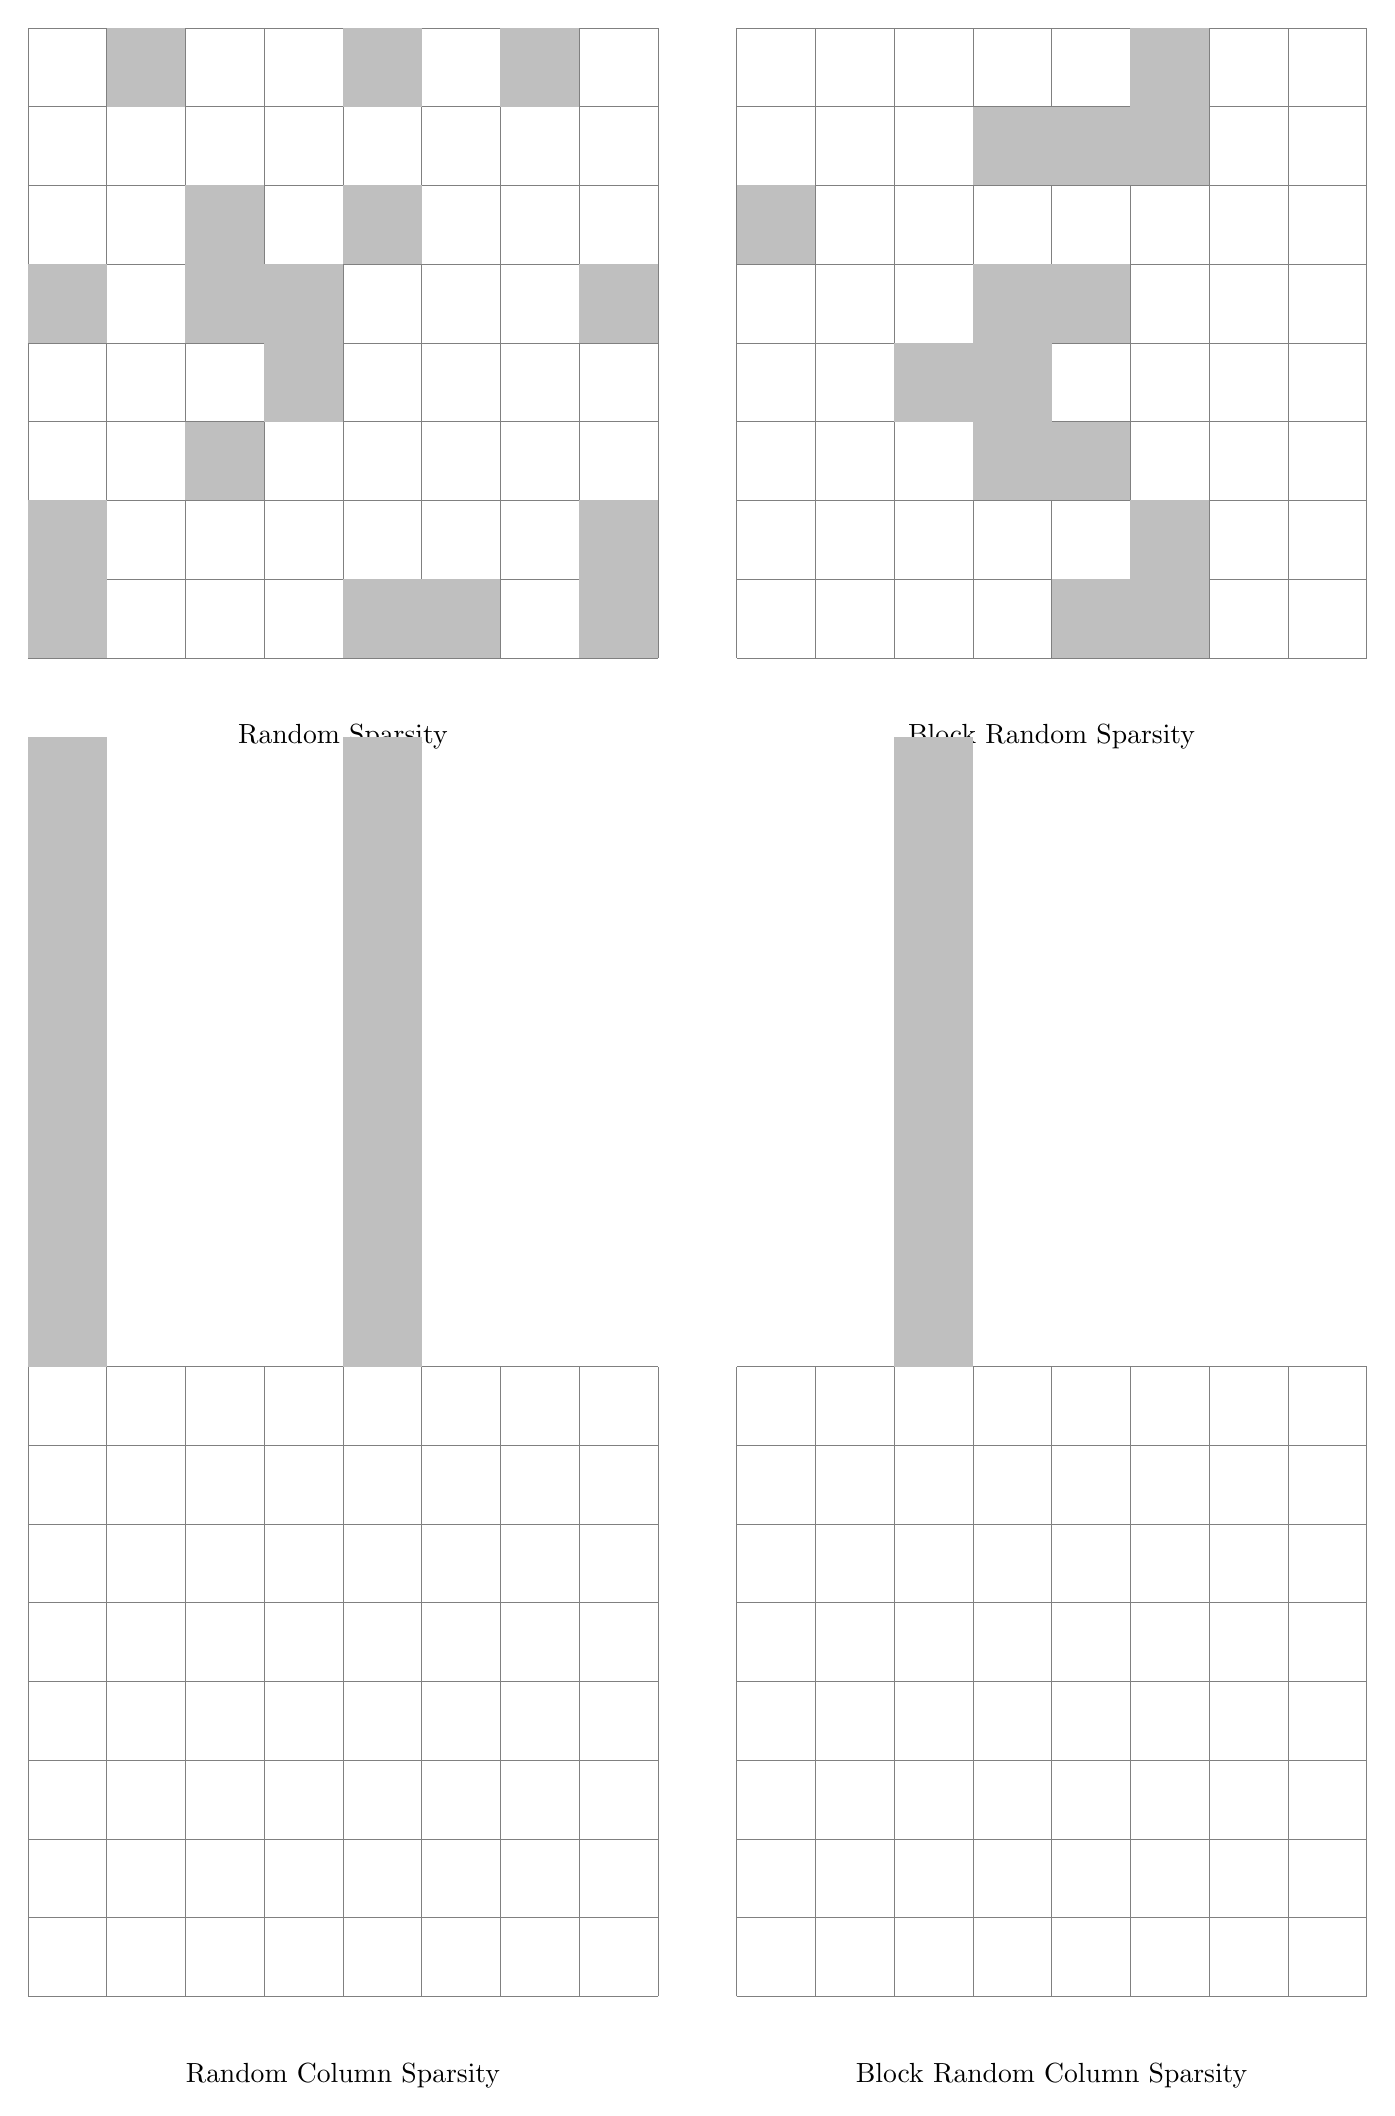
\begin{tikzpicture}[every node/.style={inner sep=0,outer sep=0}]
  % Draw the grid
  \draw[help lines,step=1cm] (0,0) grid (8,8);

  % Place sparsity patterns
  \pic at (0,0) {random};
  \node at (4,-1) {Random Sparsity};

  \draw[help lines,step=1cm] (9,0) grid (17,8);
  \pic at (9,0) {block-random};
  \node at (13,-1) {Block Random Sparsity};

  \draw[help lines,step=1cm] (0,-9) grid (8,-17);
  \pic at (0,-9) {random-column};
  \node at (4,-18) {Random Column Sparsity};

  \draw[help lines,step=1cm] (9,-9) grid (17,-17);
  \pic at (9,-9) {block-column-random};
  \node at (13,-18) {Block Random Column Sparsity};
\end{tikzpicture}
\end{document}